In this part of my thesis I report the results from my experiments. Since there are no direct benchmarks it's important to know how to view the results. In the simplest form successful results can be stated when betting is profitable, which some of the models were able to achieve. Unfortunately this is very narrow perspective and for that reason in this part of my thesis I will dig deeper to see why some of the models were able to achieve profitable returns and what downsides these models and strategies might have even though they were profitable. Also, it's important to see how valuable the novel EA Sport's video game series FIFA's player attribute dataset is for the prediction.

\section{Results from tournament simulations}
Tournament simulation results for each of the models are listed in the tables \ref{table:outcomemodel}, \ref{table:scoreresults}, \ref{table:onevsrestresults} and \ref{table:linearmodel}. Tables includes metrics for accuracy, log loss, unit strategy's profit and kelly strategy's profit. Listed values are averages from 10 individual simulations and include standard deviation. All metrics are listed for every feature set used to train the model. In depth details for each feature set are listed in the table \ref{table:featuresetlist}.

First of all it's important to see if any of the models was able to generate profit. Preferably model should be profitable in each of the tournaments, since investor prefer steady profits. Also, being always profitable is an indicator goodness-of-fit. If model is able to capture the logic from different data periods and estimate correctly based on that it's harder to say that the model was just lucky all the time. Based on unit profit \textit{Outcome mode}, \textit{Score model} and \textit{OVR model} are can be profitable in every tournament, but not with all feature sets.  Good unit profits and high accuracy go hand in hand, which is no surprise, but high accuracy is not a clear indicator for good kelly profits, which is a slight of a surprise. For this reason not all of these models are able to be generate positive returns with using kelly as betting strategy. In fact only \textit{Outcome model}, trained with player features, is the only model that can be profitable using both of the strategies. To compare model's accuracy we can use bookmaker's odds to form a comparison model. Using bookmaker's average odds their accuracy on World cup 2018 and 2014 was 56.25\% (36 games correctly predicted) and 51.5625 (33 games correctly predicted) \% on 2010. Most of the models are better in accuracy. This means that the models' predictions are not just better than random but even better than the market's average predictions are.

But which of the feature set and model combinations is the best? This question is tricky to answer. If being profitability in every tournament with high profit is preferred than \textit{Score model}, trained with all features, might be the right choice. Whereas highest unit profits are achieved with \textit{OVR model} trained with player features. Using only these metrics to validate is a model good enough to be trusted in the next World cup 2022 is too risky. Being profitable in 192 games (64 per three tournaments) is a good start, but it's also important to understand how the models predict individual games to understand the total profits better.

\begin{table}
    \caption{Feature set description}
    \begin{tabular}{| c | c|}
        \hline
        Feature set's name & Description \\
        \hline
        Player features & FIFA player attributes only \\
        All Features & General features and Player features \\
        General Features & All excluding Player features \\
        \hline
    \end{tabular}
    \label{table:featuresetlist}
\end{table}

\begin{table}
    \caption{Tournament characteristics. Underdog victory is a case where the winning team has higher odds for winning then the other team.}
    \begin{tabular}{| c | c|c | c|}
        \hline
        Characteristic & \textbf{WC 2018} & \textbf{WC 2014} & \textbf{WC 2010}\\
        \hline
        Home wins & 25 & 28 & 24\\
        Draws & 14 & 13 & 16\\
        Away wins & 25 & 23 & 24\\
        Underdog victory  & 14 & 15 & 14\\
        \hline
    \end{tabular}
    \label{table:tournamentcharacteristics}
\end{table}


\begin{table}
    \caption{Results for Outcome model}
    \begin{tabular}{| c  c| c| c| c|c|}
        \hline
        Metric& & \textbf{WC 2018} & \textbf{WC 2014} & \textbf{WC 2010} & Mean\\
        \hline
        Accuracy & AF & 57.34\% $\pm$ 0.72 & 60.94\% $\pm$ 1.71 & 54.84\% $\pm$ 1.09& 57.71 \\
         & GF & 52.03\% $\pm$ 1.22 & 56.56\% $\pm$ 0.62 & 55.47\% $\pm$ 1.05& 54.69 \\
         & PF & 60.47\% $\pm$ 1.41 & 59.69\% $\pm$ 0.94 & 54.22\% $\pm$ 2.22& 58.13 \\
         & & & & & \\
        Log Loss & AF & 0.9673 $\pm$ 0.0037 & 0.9362 $\pm$ 0.0047 & 0.9922 $\pm$ 0.0075& 0.9652 \\
         & GF & 1.0122 $\pm$ 0.0045 & 0.9549 $\pm$ 0.0053 & 0.9676 $\pm$ 0.0052& 0.9782 \\
         & PF & 0.9406 $\pm$ 0.0026 & 0.9503 $\pm$ 0.0024 & 1.0118 $\pm$ 0.0045& 0.9676 \\
         & & & & & \\
        Unit profit & AF & 6.39\% $\pm$ 1.96 & 15.65\% $\pm$ 5.21 & 2.93\% $\pm$ 4.43& 8.32 \\
         & GF & -3.48\% $\pm$ 3.4 & 5.17\% $\pm$ 1.52 & 5.04\% $\pm$ 3.67& 2.24 \\
         & PF & 18.38\% $\pm$ 4.26 & 12.72\% $\pm$ 2.22 & 3.32\% $\pm$ 8.33& 11.47 \\
         & & & & & \\
        Kelly profit & AF & -10.58\% $\pm$ 7.01 & 18.55\% $\pm$ 10.13 & 23.26\% $\pm$ 18.96& 10.41 \\
         & GF & -47.32\% $\pm$ 4.1 & 2.86\% $\pm$ 8.15 & 48.9\% $\pm$ 16.64& 1.48 \\
         & PF & 46.63\% $\pm$ 8.79 & 12.26\% $\pm$ 6.57 & 2.75\% $\pm$ 9.05& 20.55 \\
 \hline
    \end{tabular}
    \label{table:outcomemodel}
\end{table}


\begin{table}
    \caption{Results for Score model}
    \begin{tabular}{| c  c| c| c| c|c|}
        \hline
        Metric& & \textbf{WC 2018} & \textbf{WC 2014} & \textbf{WC 2010} & Mean\\
        \hline
        Accuracy & AF & 59.38\% $\pm$ 0.0 & 58.13\% $\pm$ 0.62 & 52.81\% $\pm$ 0.62& 56.77 \\
         & GF & 52.03\% $\pm$ 1.0 & 59.38\% $\pm$ 0.0 & 50.94\% $\pm$ 0.77& 54.12 \\
         & PF & 58.44\% $\pm$ 1.74 & 61.09\% $\pm$ 0.84 & 53.91\% $\pm$ 0.78& 57.81 \\
         & & & & & \\
        Log Loss & AF & 0.9508 $\pm$ 0.0016 & 0.935 $\pm$ 0.0005 & 0.9788 $\pm$ 0.0016& 0.9549 \\
         & GF & 0.9831 $\pm$ 0.0012 & 0.9133 $\pm$ 0.0011 & 0.9522 $\pm$ 0.001& 0.9495 \\
         & PF & 0.9566 $\pm$ 0.0013 & 0.9446 $\pm$ 0.0024 & 0.9996 $\pm$ 0.0009& 0.9669 \\
         & & & & & \\
        Unit profit & AF & 13.52\% $\pm$ 0.0 & 5.94\% $\pm$ 2.11 & -2.8\% $\pm$ 1.29& 5.55 \\
         & GF & -5.4\% $\pm$ 2.57 & 13.66\% $\pm$ 0.0 & -5.08\% $\pm$ 2.45& 1.06 \\
         & PF & 12.26\% $\pm$ 5.1 & 16.11\% $\pm$ 2.64 & 2.23\% $\pm$ 2.09& 10.2 \\
         & & & & & \\
        Kelly profit & AF & 35.59\% $\pm$ 4.45 & 12.37\% $\pm$ 1.02 & 24.2\% $\pm$ 4.43& 24.05 \\
         & GF & -19.06\% $\pm$ 1.87 & 107.61\% $\pm$ 4.47 & 99.75\% $\pm$ 3.63& 62.77 \\
         & PF & 2.04\% $\pm$ 2.62 & 10.82\% $\pm$ 4.87 & 8.3\% $\pm$ 2.1& 7.05 \\
 \hline
    \end{tabular}
    \label{table:scoreresults}
\end{table}

\begin{table}
    \caption{Results for OneVsRest model}
    \begin{tabular}{| c  c| c| c| c|c|}
        \hline
        Metric& & \textbf{WC 2018} & \textbf{WC 2014} & \textbf{WC 2010} & Mean\\
        \hline
        Accuracy & AF & 57.66\% $\pm$ 0.47 & 57.34\% $\pm$ 1.22 & 56.09\% $\pm$ 0.84& 57.03 \\
         & GF & 51.25\% $\pm$ 1.95 & 55.16\% $\pm$ 1.57 & 57.03\% $\pm$ 1.05& 54.48 \\
         & PF & 61.09\% $\pm$ 1.3 & 60.16\% $\pm$ 1.05 & 54.37\% $\pm$ 1.36& 58.54 \\
         & & & & & \\
        Log Loss & AF & 0.9646 $\pm$ 0.0035 & 0.9382 $\pm$ 0.0039 & 0.9831 $\pm$ 0.005& 0.962 \\
         & GF & 1.012 $\pm$ 0.0052 & 0.9515 $\pm$ 0.0068 & 0.9583 $\pm$ 0.0059& 0.9739 \\
         & PF & 0.9365 $\pm$ 0.0023 & 0.9564 $\pm$ 0.0032 & 1.0083 $\pm$ 0.0052& 0.9671 \\
         & & & & & \\
        Unit profit & AF & 7.31\% $\pm$ 1.04 & 5.01\% $\pm$ 2.93 & 6.52\% $\pm$ 2.97& 6.28 \\
         & GF & -5.03\% $\pm$ 4.84 & 3.04\% $\pm$ 4.31 & 10.38\% $\pm$ 3.38& 2.8 \\
         & PF & 19.83\% $\pm$ 4.01 & 14.14\% $\pm$ 2.82 & 3.88\% $\pm$ 5.11& 12.62 \\
         & & & & &  \\
        Kelly profit & AF & -2.6\% $\pm$ 6.57 & 9.34\% $\pm$ 8.69 & 26.26\% $\pm$ 10.92& 11.0 \\
         & GF & -44.81\% $\pm$ 3.96 & 14.61\% $\pm$ 13.1 & 83.44\% $\pm$ 23.89& 17.75 \\
         & PF & 61.65\% $\pm$ 9.88 & -3.92\% $\pm$ 4.68 & 0.77\% $\pm$ 7.02& 19.5 \\
 \hline
    \end{tabular}
    \label{table:onevsrestresults}
\end{table}

\begin{table}
    \caption{Results for Logistic Regression model}
    \begin{tabular}{| c  c| c| c| c|c|}
        \hline
        Metric & & \textbf{WC 2018} & \textbf{WC 2014} & \textbf{WC 2010}& Mean\\
        \hline
        Accuracy & AF & 54.84\% $\pm$ 0.84 & 63.59\% $\pm$ 0.72 & 51.41\% $\pm$ 1.3& 56.61 \\
         & GF & 51.72\% $\pm$ 1.09 & 63.28\% $\pm$ 1.26 & 54.37\% $\pm$ 1.53& 56.46 \\
         & PF & 59.69\% $\pm$ 0.62 & 62.19\% $\pm$ 0.62 & 50.78\% $\pm$ 0.78& 57.55 \\
         & & & & & \\
        Log Loss & AF & 0.9719 $\pm$ 0.0043 & 0.8791 $\pm$ 0.0025 & 1.0418 $\pm$ 0.0071& 0.9643 \\
         & GF & 0.9953 $\pm$ 0.0041 & 0.9112 $\pm$ 0.0035 & 0.9837 $\pm$ 0.0028& 0.9634 \\
         & PF & 0.9334 $\pm$ 0.0017 & 0.9311 $\pm$ 0.0032 & 1.0563 $\pm$ 0.0064& 0.9736 \\
         & & & & & \\
        Unit profit & AF & 0.79\% $\pm$ 1.51 & 27.73\% $\pm$ 3.09 & -5.11\% $\pm$ 3.88& 7.8 \\
         & GF & -3.75\% $\pm$ 2.07 & 24.57\% $\pm$ 4.51 & -0.28\% $\pm$ 5.87& 6.85 \\
         & PF & 14.73\% $\pm$ 1.93 & 21.98\% $\pm$ 2.7 & -8.95\% $\pm$ 2.03& 9.25 \\
         & & & & & \\
        Kelly profit & AF & -20.29\% $\pm$ 5.49 & 271.57\% $\pm$ 25.03 & -43.87\% $\pm$ 5.37& 69.14 \\
         & GF & -36.47\% $\pm$ 3.66 & 125.73\% $\pm$ 11.94 & 8.75\% $\pm$ 10.44& 32.67 \\
         & PF & 55.93\% $\pm$ 4.8 & 52.77\% $\pm$ 8.74 & -49.56\% $\pm$ 4.26& 19.71 \\
 \hline
    \end{tabular}
    \label{table:linearmodel}
\end{table}

\section{How models differ in game-level predictions?}
To understand the tournament simulation results better it's important to understand what happens in the game-level predictions. Comparing all the tournaments at game-level is not feasible. For this reason I chose use World cup 2018 for game-level simulation. This should be ok, since tournaments have similar characteristics, which are listed in the table \ref{table:tournamentcharacteristics}. The only noteworthy difference might be the higher number of games ending at draw in World cup 2010.

The reason why tournament with few more games ending at draw matters so much is because models are very inaccurate when it comes to predicting the outcome of a draw. For example the average precision for \textit{Outcome model} with any of the feature sets is at maximum 0.1. The average recall is at best 0.00625. In most of the cases precision and recall are almost always zero. Both of those values were for World Cup 2010, meaning that only one draw from the 10 draws that were predicted in total was correct. Predicting draws is hard since football games often have low scores. A goal for the underdog is very valuable but not that unlikely to do. This makes winning the game for the favourite team significantly harder. Draws are not preferred by the bookmakers either. Very seldom draw has the lowest odds. For example only one game in World Cup 2010 had the lowest odds for draw and that game didn't end as draw.

Since tournaments' characteristics are similar enough I can assume that I can use any of the tournaments to compare game-level characteristics of my models. I will use the World cup 2018 with all of the available features to compere models against each other.

I compared simulation results from all of the models for World cup 2018. Models were trained using all of the available features. One interesting fact is that models predict outcomes very similarly as figure \ref{fig:unit_model_comparison} shows. Outcome and score model almost equal in their predictions. Based on the overall results models should differ more, since profits are not equal or even similar. What might be the reason for this? To see more details it's wise to use the kelly strategy's cash balance progression from the figure \ref{fig:kelly_model_comparison} to compare the models. Cash balances clearly develop out of phase from the first game onward. Reason behind this is different probability distributions that the models output. By observing the tables \ref{table:home_win_metrics}, \ref{table:draw_metrics} and \ref{table:away_win_metrics} we can see that models' behaviour is fairly similar with probability prediction of home win and away win, but differs clearly with draw prediction. Even when only random forest based solutions are compared the difference between the models is most obvious when probability estimates for draw are compared. The figure \ref{fig:draw_probability} shows how differently the models estimate the probability of game ending in draw. This figure backed by the standard deviation values from the table \ref{table:draw_metrics} shows that \textit{Outcome model} and \textit{OVR model} predict draw probabilities more aggressively; both models sometimes predict lot lower or higher probabilities than rest of the models. \textit{Score model} and \textit{Linear model} have significantly lower standard deviation than \textit{Outcome model} or \textit{OVR model}. Since averages from all of the models are quite close this means that \textit{Score model} and \textit{Linear model} have more stable predictions. With low correlation to rest of the models \textit{linear model} is the most independent with its probability estimates. Since there are no true probabilities available for game ending in draw it's hard to say what is the better way to estimate probability of a draw; is the true probability for every game closer to the average value or should model be more aggressive with the estimates. When current results are viewed less varying probability estimates for draw might be a better option since \textit{Score model} is able to make profit with two different feature sets while \textit{Outcome model} and \textit{OVR model} are not. To have some kind of idea what the probability distribution of draw based on elo rating difference is, I split elo rating difference range to deciles and calculated how many games ended in that decile ended in draw. Results for this are in the figure \ref{fig:draw_prob_dist}. Based on this figure ending in draw is not random and the bigger the difference between elo ratings is the more probable it's that game will not end in draw.

\begin{table}[h]
    \caption{Means, standard deviations, and correlations of home win probability predictions for World cup 2018.}
    \label{table:home_win_metrics}
    \noindent
    \begin{tabular}{c c c c c c c c c c}
    \toprule
    & Measure
      & \multicolumn{1}{r}{mean}
      & \multicolumn{1}{c}{sd}
      & \multicolumn{4}{c@{}}{correlations}\\
    \cmidrule(l){5-8}
    & & & & \multicolumn{1}{c}{1{.}}
          & \multicolumn{1}{c}{2{.}}
          & \multicolumn{1}{c}{3{.}}
          & \multicolumn{1}{c@{}}{4{.}}\\
    \midrule
    & Models \\
    1{.} & Score     &   0.3956 &   0.1588 \\
    2{.} & Outcome   &   0.3854 &   0.1685 & 0.9873  \\
    3{.} & OneVsRest &   0.4016 &   0.1687 & 0.9870 &  0.9871  & \\
    4{.} & Linear    &   0.4170 & 0.1698   & 0.9654 & 0.9660   &  0.9733 \\
    \bottomrule
    \end{tabular}
    \end{table}

    \begin{table}[h]
    \caption{Means, standard deviations, and correlations of draw probability predictions for World cup 2018.}
    \label{table:draw_metrics}
    \noindent
    \begin{tabular}{c c c c c c c c c c}
    \toprule
    & Measure
      & \multicolumn{1}{r}{mean}
      & \multicolumn{1}{c}{sd}
      & \multicolumn{4}{c@{}}{correlations}\\
    \cmidrule(l){5-8}
    & & & & \multicolumn{1}{c}{1{.}}
          & \multicolumn{1}{c}{2{.}}
          & \multicolumn{1}{c}{3{.}}
          & \multicolumn{1}{c@{}}{4{.}}\\
    \midrule
    & Models \\
    1{.} & Score     &   0.2527 &   0.0274 \\
    2{.} & Outcome   &   0.2619 &   0.0414 & 0.8102  \\
    3{.} & OneVsRest &   0.2553 &   0.0414 & 0.7713  &  0.9333  & \\
    4{.} & Linear    &   0.2484 &   0.0197 & 0.2356  &  0.3162  &  0.3080 \\
    \bottomrule
    \end{tabular}
    \end{table}

    \begin{table}[h]
    \caption{Means, standard deviations, and correlations of away win probability predictions for World cup 2018.}
    \label{table:away_win_metrics}
    \noindent
    \begin{tabular}{c c c c c c c c c c}
    \toprule
    & Measure
      & \multicolumn{1}{r}{mean}
      & \multicolumn{1}{c}{sd}
      & \multicolumn{4}{c@{}}{correlations}\\
    \cmidrule(l){5-8}
    & & & & \multicolumn{1}{c}{1{.}}
          & \multicolumn{1}{c}{2{.}}
          & \multicolumn{1}{c}{3{.}}
          & \multicolumn{1}{c@{}}{4{.}}\\
    \midrule
    & Models \\
    1{.} & Score     &   0.3517 &   0.1504 \\
    2{.} & Outcome   &   0.3528 &   0.1667 & 0.9824  \\
    3{.} & OneVsRest &   0.3431 &  0.1674  & 0.9814  &  0.9889  & \\
    4{.} & Linear    &   0.3345 &  0.1753  & 0.9648  & 0.9672   &  0.9680 \\
    \bottomrule
    \end{tabular}
    \end{table}
\begin{figure}[H]
    \centering
    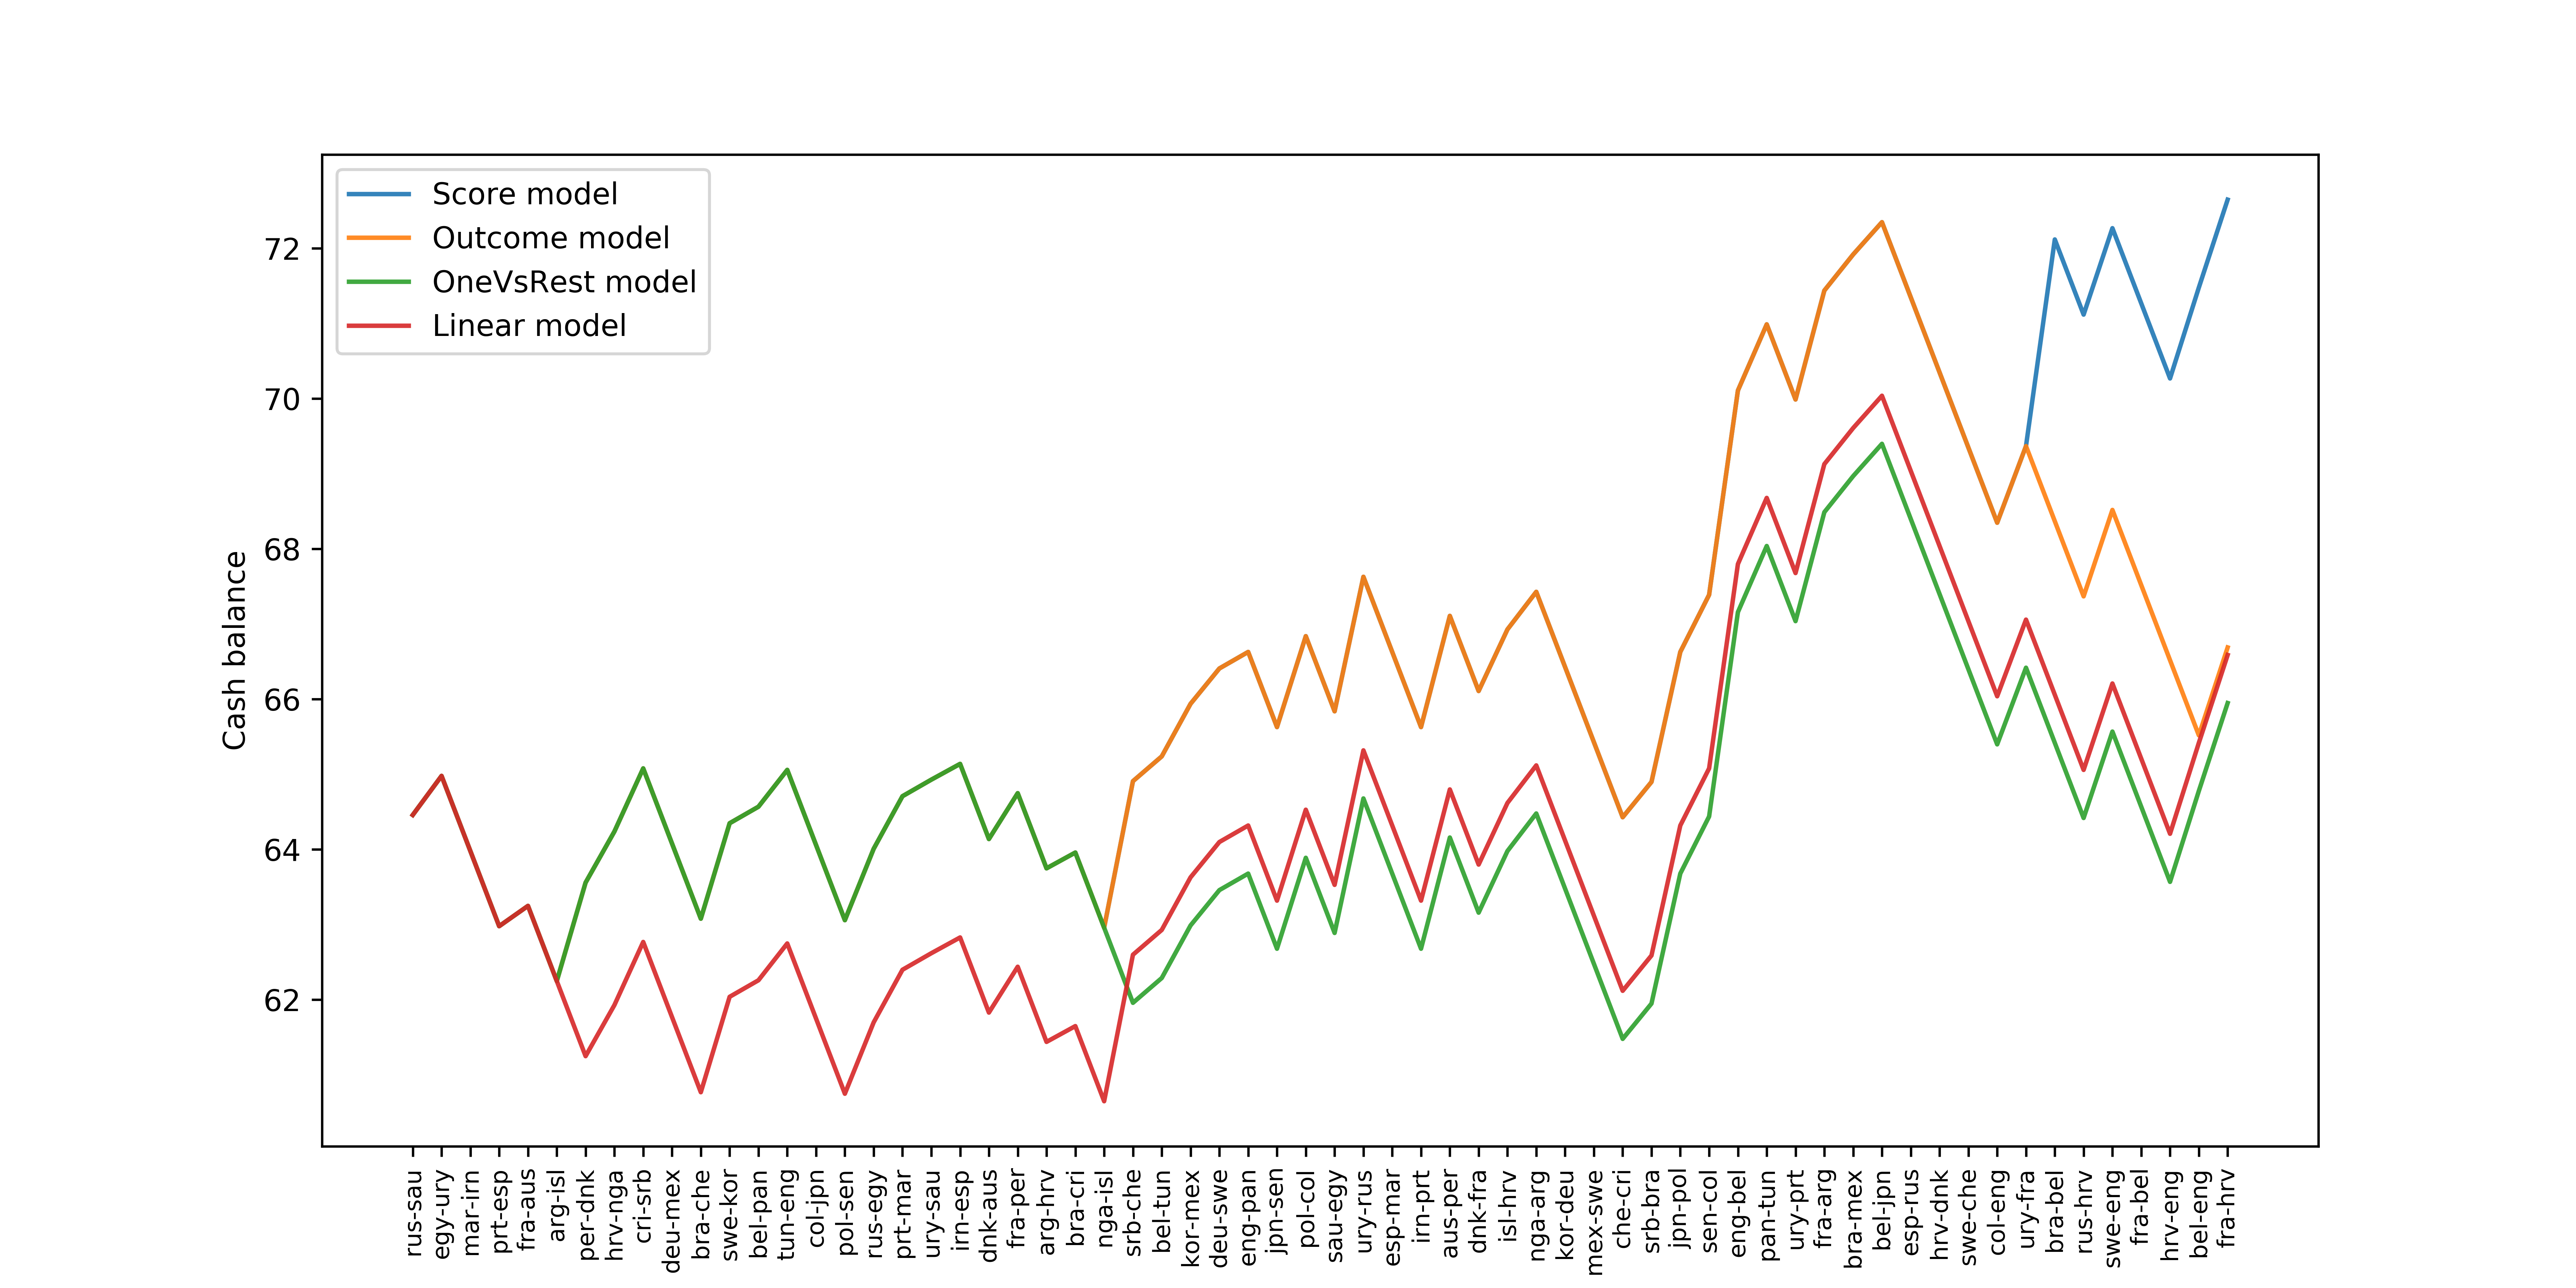
\includegraphics[width=0.7\textwidth]{img/match_level_2018_model_unit.png}
    \caption{Unit strategy's cash balance progression on World Cup 2018.}
    \label{fig:unit_model_comparison}
\end{figure}

\begin{figure}[H]
    \centering
    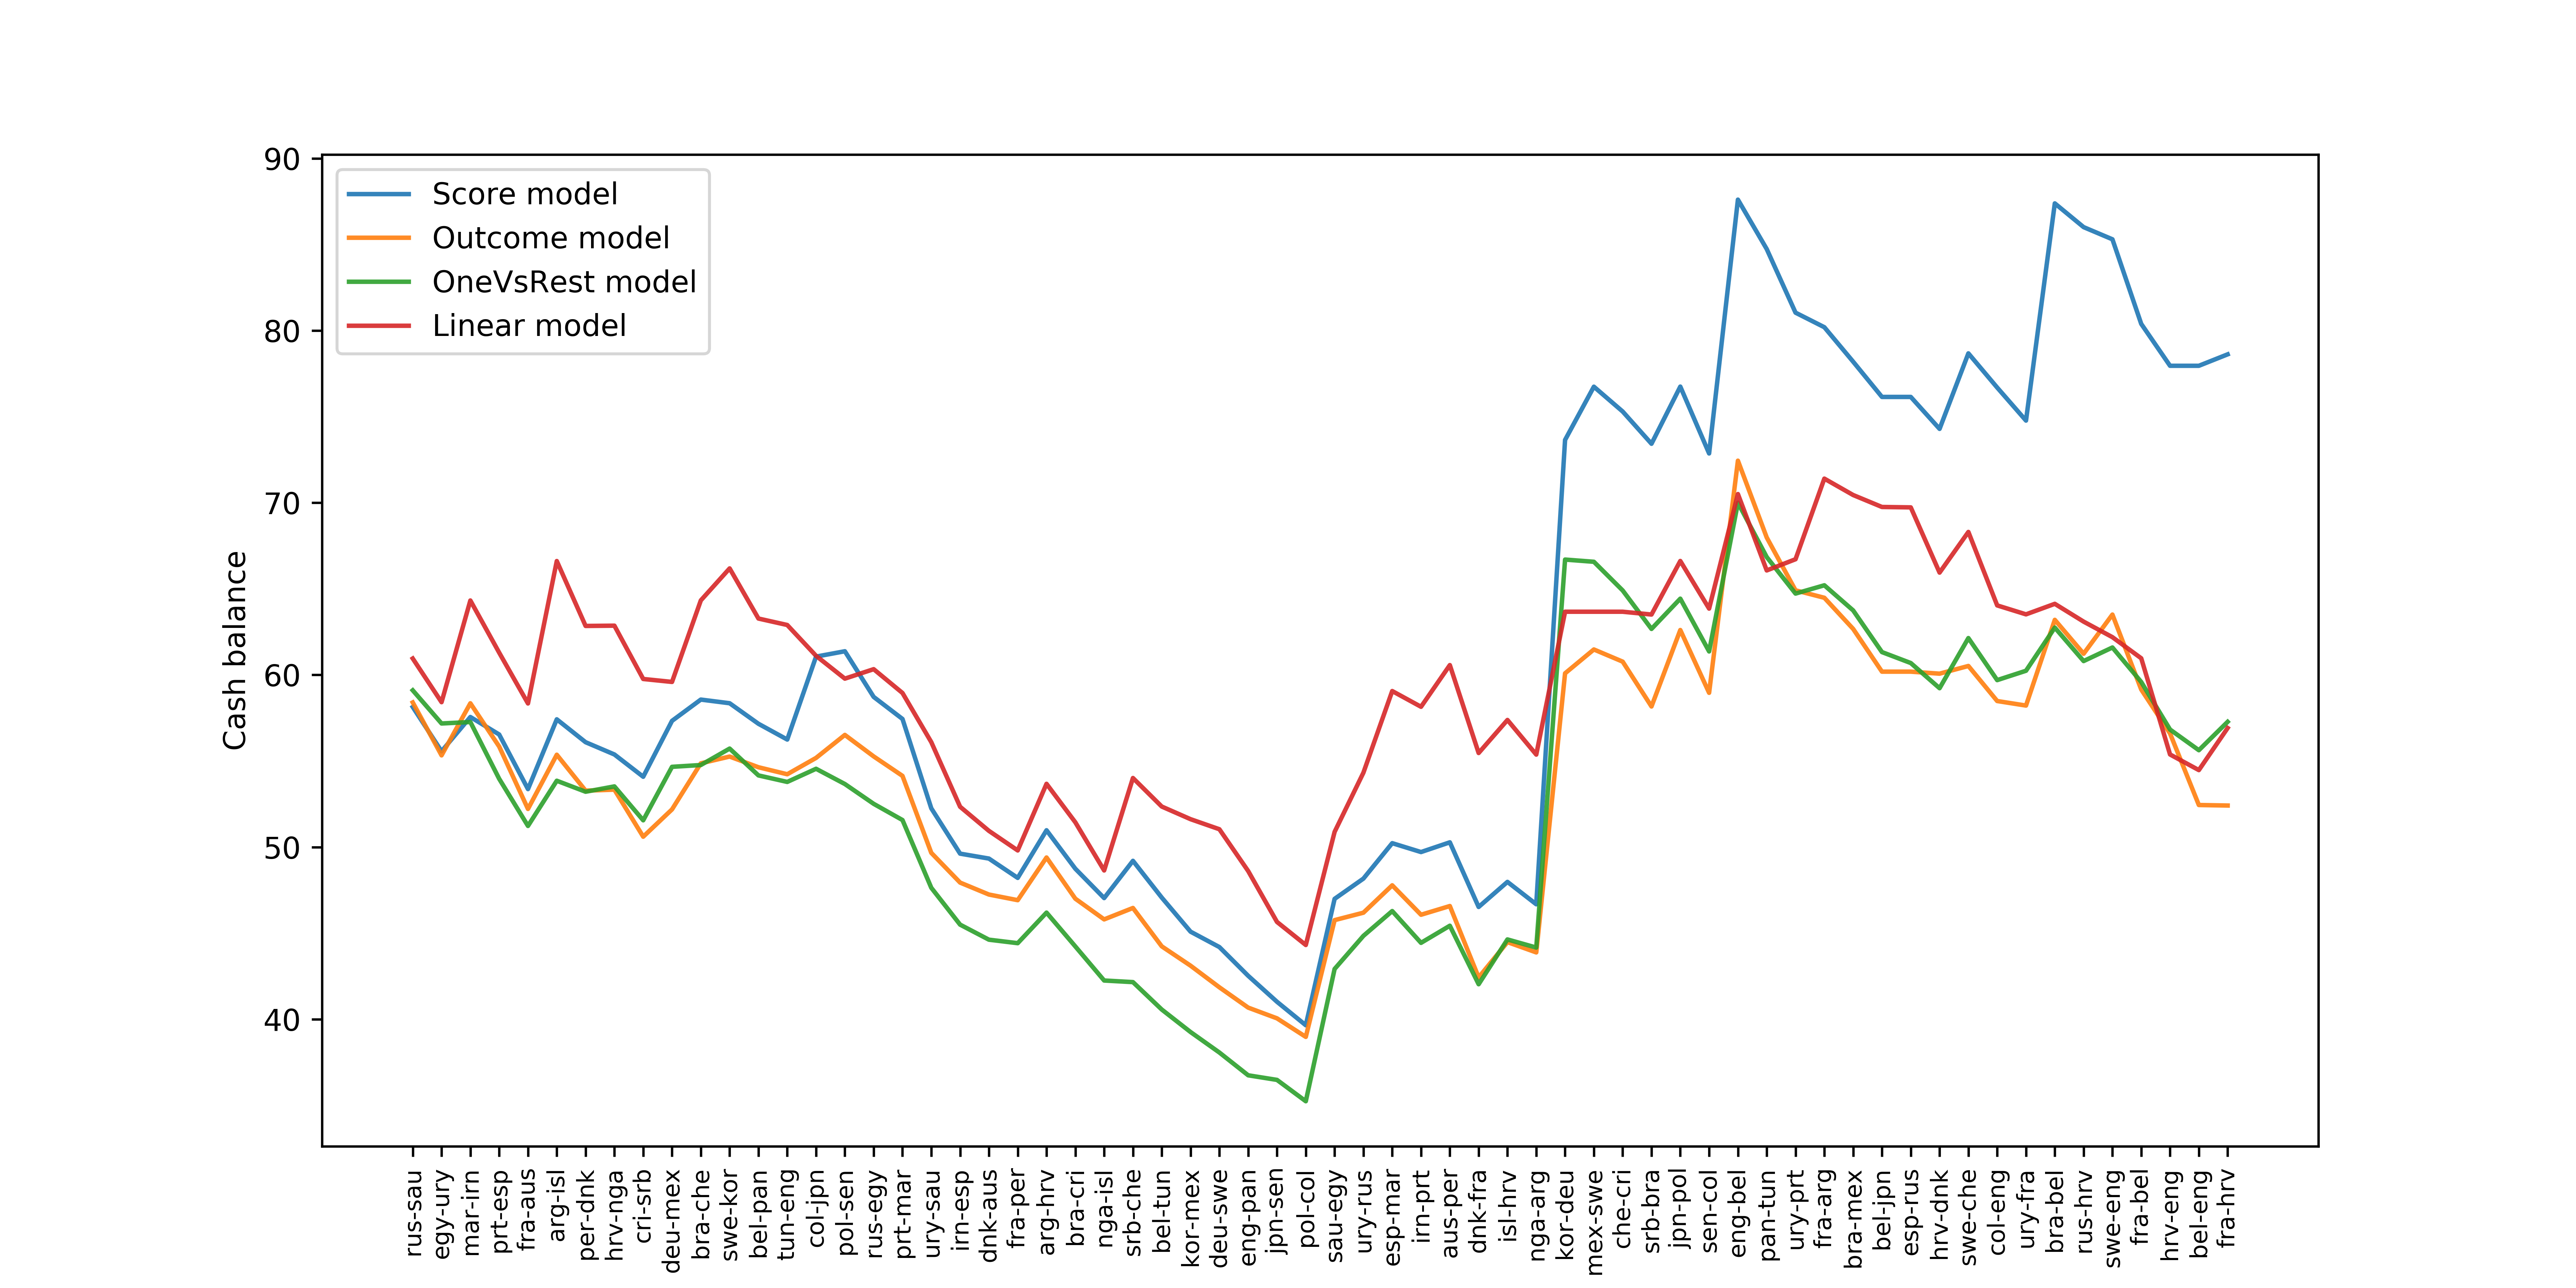
\includegraphics[width=0.7\textwidth]{img/match_level_2018_model_kelly.png}
    \caption{Kelly strategy's cash balance progression on World Cup 2018.}
    \label{fig:kelly_model_comparison}
\end{figure}

\begin{figure}[H]
    \centering
    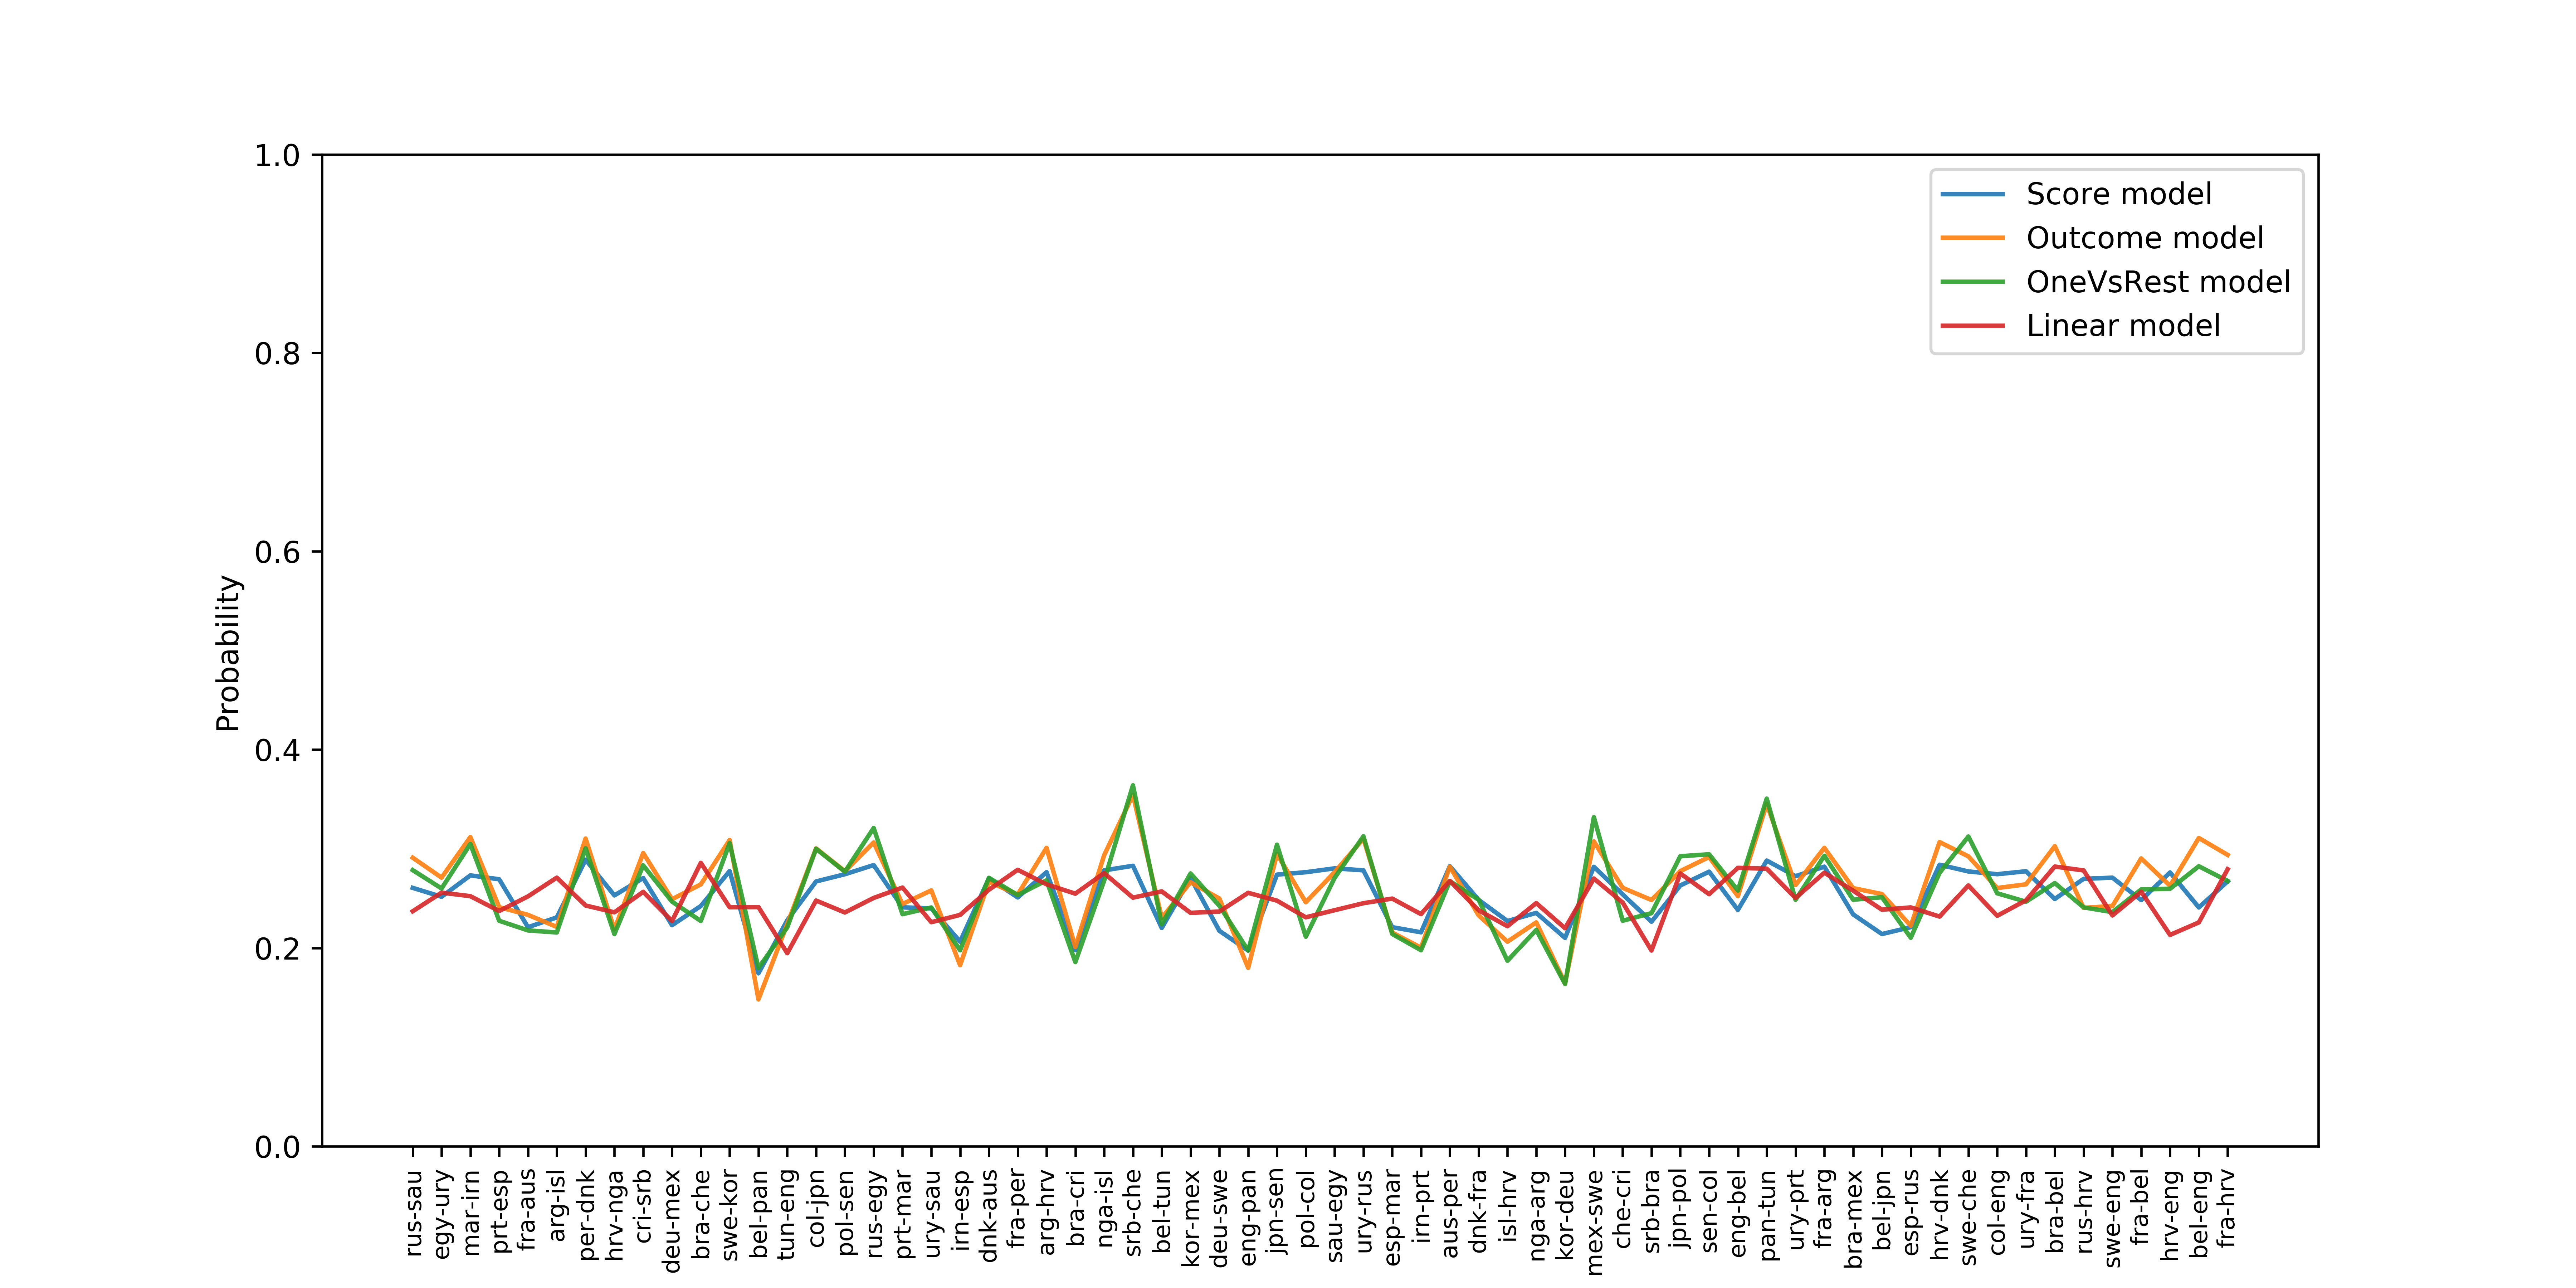
\includegraphics[width=0.7\textwidth]{img/match_level_2018_model_probability_draw_prob.png}
    \caption{Predicted probability of draw in the World Cup 2018.}
    \label{fig:draw_probability}
\end{figure}

\begin{figure}[H]
    \centering
    \includegraphics[width=0.7\textwidth]{img/draw_true_probability.eps}
    \caption{Probability distribution of game ending in draw given elo rating difference.}
    \label{fig:draw_prob_dist}
\end{figure}


\section{Feature set differences}
It's interesting that narrower feature sets can produce better accuracy. How can less describe more? It's against common sense, right?

These problems are visible if models' accuracy is compared. Being one of the most important metrics, it's still not the most important for the sophisticated betting strategies like kelly, which utilizes model's probability estimates. Log loss
is a metric that can be used to compare probability distributions' accuracy. A smaller value indicates a more accurate estimate. When log loss is compared per tournament model trained with limited feature set can have lower log loss value than the same model that is trained using all of the features. But when average performance from every tournament is considered training model with all features seems to output the lowest log loss score with \textit{Outcome model} and \textit{OVR model} and second lowest (only 0.0009 difference at highest) with \textit{Score model} and \textit{Linear model}. This indicates that even-though increasing accuracy might not benefit from using all features probability distribution prediction clearly benefits. Since football games often have low scores can last minute surprises change the whole game. Underdog can beat the favourite or at least square the game. This means that achieving high accuracy is hard, but fixing probabilities to match the true ones has more room to improve.

Random forest includes the information on feature importance. These values can give insight on models reasoning. This data combined with optimal hyperparameters is one way to interpret the models since inspecting every single tree in the forest would be too cumbersome. Segal \cite{segal2004machine} showed that noisy variable can lead to higher optimal value for minimum samples at leaf hyperparameter. With generic features models seem to prefer higher value for the hyperparameter minimum samples at leaf as we can see from the table \ref{table:hyperparam_results}.  Figure \ref{fig:outcome_feature_importance_gf} lists feature's importance for Outcome model trained with generic features. Difference between elo rating dominates the others, but just by looking at the plot it's impossible to say if any of the features could be considered to be just noise. Lower importance features like \textit{home\_goal} and \textit{away\_goal} seem to be in the middle tier when model is trained with all features. This higher importance compared to other features could mean that these features have predicting power. Comparing figures \ref{fig:outcome_feature_importance_af}, \ref{fig:outcome_feature_importance_gf} and \ref{fig:outcome_feature_importance_pf} only confirms that elo is very important feature and shows that some of the player attributes rank high. So it's clear what features are important but not that clear what features are unimportant - if any of them are.

\begin{table}
    \caption{Hyperparameter selection results for random forest models.}
    \begin{tabular}{| c  c| c| c| c|}
        \hline
        Model & Features & \# of predictors & Min samples at leaf & Max depth\\
        \hline
        Score & AF & $\sqrt{M}$ & 1 & 8 \\
         & GF & $\log_2{M}$ & 10 & 8 \\
         & PF & $\sqrt{M}$ & 5 & Na \\
         \hline
        Outcome & AF & $\sqrt{M}$ & 3 & 8 \\
         & GF & $\log_2{M}$ & 15 & 5 \\
         & PF & $\log_2{M}$ & 3 & 8 \\
        \hline
        OVR & AF home win & $\sqrt{M}$ & 3 & 5 \\
        OVR & AF draw & $\sqrt{M}$ & 5 & Na \\
        OVR & AF away win & $\sqrt{M}$ & 3 & 5 \\
        OVR & GF home win & $\sqrt{M}$ & 10 & 12 \\
        OVR & GF draw & $\log_2{M}$ & 15 & 8 \\
        OVR & GF away win & $\log_2{M}$ & 10 & 5 \\
        OVR & PF home win & $\log_2{M}$ & 3 & 5 \\
        OVR & PF draw & $\log_2{M}$ & 15 & 5 \\
        OVR & PF away win & $\log_2{M}$ & 5 & 8 \\
        \hline
    \end{tabular}
    \label{table:hyperparam_results}
\end{table}

\begin{figure}[H]
    \centering
    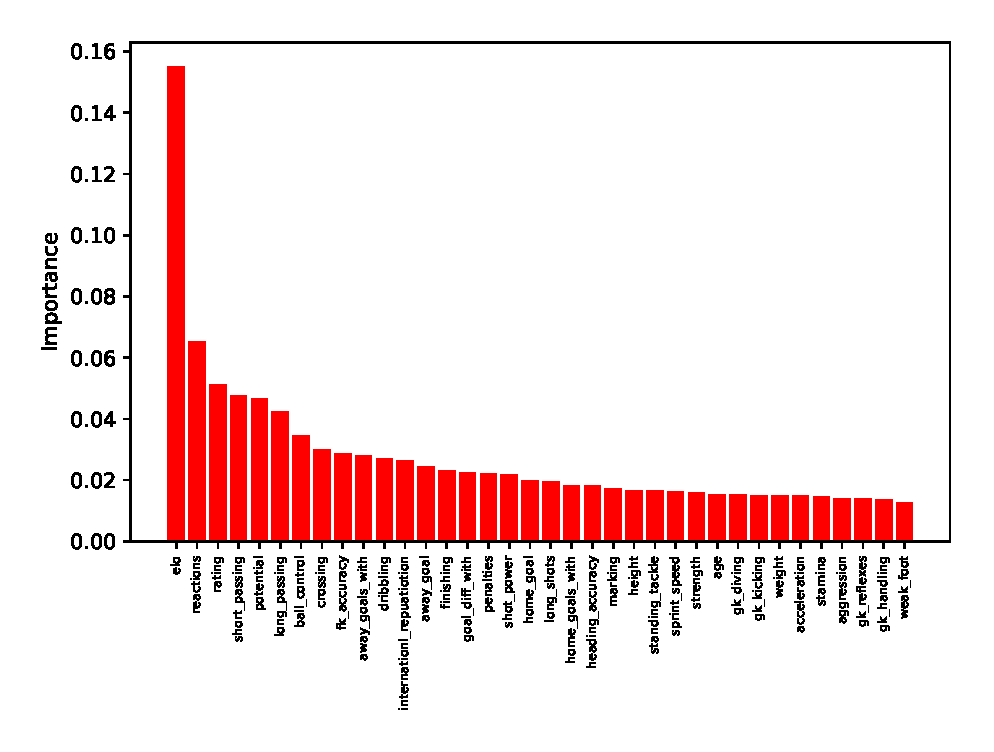
\includegraphics[width=0.7\textwidth]{img/match_level_2018_outcome_feature_importance_af_feature_importance.eps}
    \caption{Outcome model's feature importance with all features.}
    \label{fig:outcome_feature_importance_af}
\end{figure}

\begin{figure}[H]
    \centering
    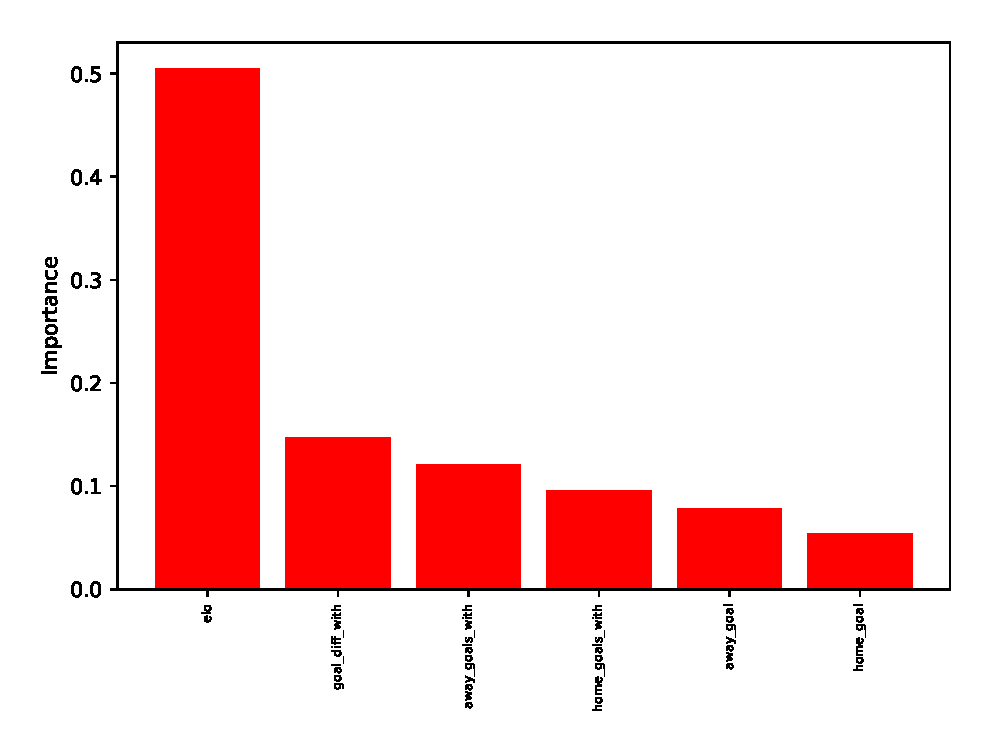
\includegraphics[width=0.7\textwidth]{img/match_level_2018_outcome_feature_importance_gf_feature_importance.eps}
    \caption{Outcome model's feature importance with generic features.}
    \label{fig:outcome_feature_importance_gf}
\end{figure}

\begin{figure}[H]
    \centering
    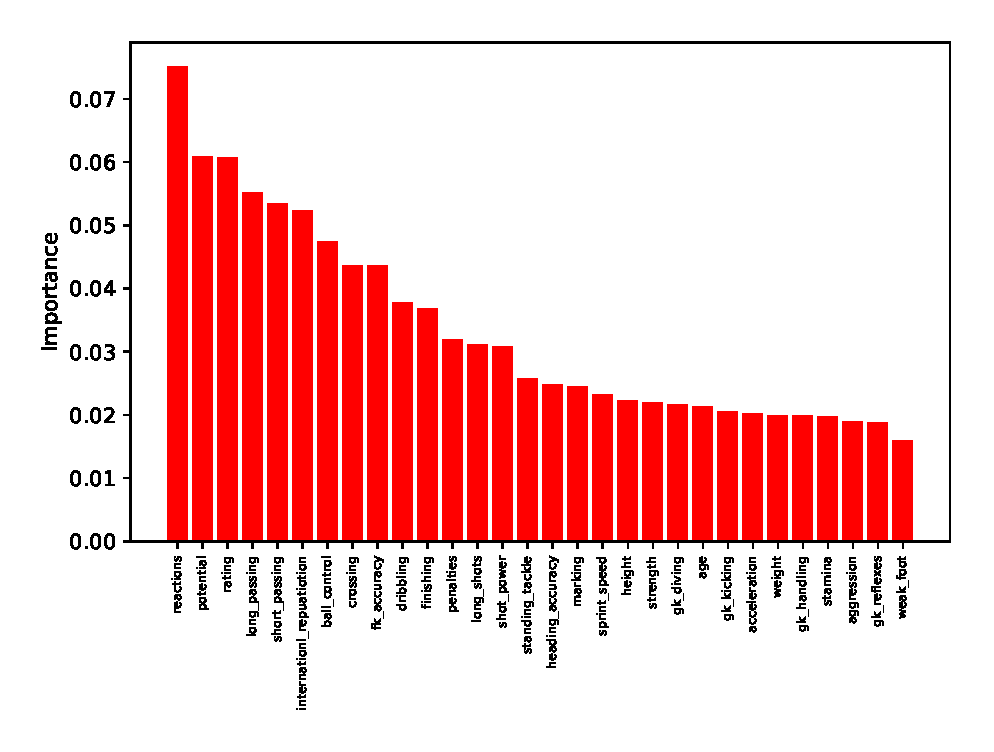
\includegraphics[width=0.7\textwidth]{img/match_level_2018_outcome_feature_importance_pf_feature_importance.eps}
    \caption{Outcome model's feature importance with player features.}
    \label{fig:outcome_feature_importance_pf}
\end{figure}

If some of the features are just noise, those features can be removed without harming the models probability estimates. One way to do this is recursive feature elimination where one by one features are eliminated and models performance is measured for every  elimination round. Test is done 100 times for every elimination round to guarantee that variation in the results won't cause feature to be eliminated to early. I did the recursive feature elimination process the \textit{Outcome model}.

\section{Recursive feature elimination}
Idea behind recursive feature elimination (RFE) is to fit the model multiple times and see which has the least amount of predictive power on average. That feature is then eliminated and process is started again until there are no features left. Average accuracy and log loss are stored for each feature set. I fitted models 100 times and used feature importance metric to compare the features. All of the feature test were done with \textit{Outcome model}.

First test included default parameters for \textit{Outcome model}: 1000 for number of estimators, number of predictors $\sqrt{}$, maximum depth Na and minimum samples at leaf 1. From figure \ref{fig:def_avg_accu} we can see that after \textit{gk\_diving} accuracy starts to decrease slowly. If we compare this result to figure \ref{fig:def_avg_loss}
it's evident that the log loss increases after \textit{gk\_diving}. For comparison I run the same test with \textit{Outcome model} using optimal parameters used in all feature setup in the table \ref{table:outcomemodel}. Results are visible in the figures \ref{fig:optimal_avg_accu} and \ref{fig:optimal_avg_loss}. With optimal hyperparameters model performs better through out the whole RFE porcess. Also, model peaks the highest accuracy with only just four features. Improvement with this same feature set is not visible in the average log loss. The average log loss has a clear performance drop only when there is a single feature left.

Since with default hyperparameters decrease in accuracy and in log loss was visible I ran the World cup simulation for \textit{Outcome model} using limited feature set that contained features: \textit{away\_goals\_with\_home, finishing\_diff, height\_diff, crossing\_diff, potential\_diff, fk\_accuracy\_diff, home\_goal\_mean, away\_goal\_mean, ball\_control\_diff, long\_passing\_diff,  short\_passing\_diff, reactions\_diff, rating\_diff, elo\_diff}. Optimal hyperparameters for this feature set are listed on the table \ref{table:hyperparam_results_rfe} and World Cup simulation results are in the table \ref{table:outcomemodel_rfe}. Based on the results model's performance according to accuracy and log loss doesn't differ significantly from the model that was trained using all features setup.

Based on the progression of average accuracy and average log loss models do not perform better when features are removed from the original feature set. Eventually performance decreases but never increases during feature elimination. Most of the time results just have natural variance, which causes small changes. It seems that using every available feature doesn't harm random forest's performance, even though there is no guarantee that all of the features are useful.
\begin{figure}[H]
    \centering
    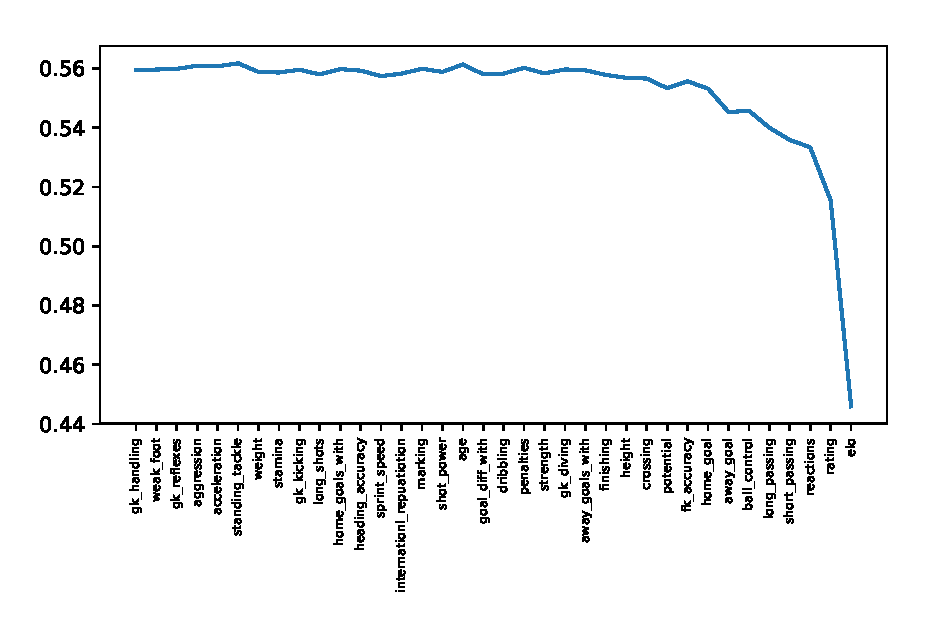
\includegraphics[width=0.7\textwidth]{img/default_avg_accuracy.eps}
    \caption{Mean accuracy for recursive feature elimination on outcome model with default parameters.}
    \label{fig:def_avg_accu}
\end{figure}

\begin{figure}[H]
    \centering
    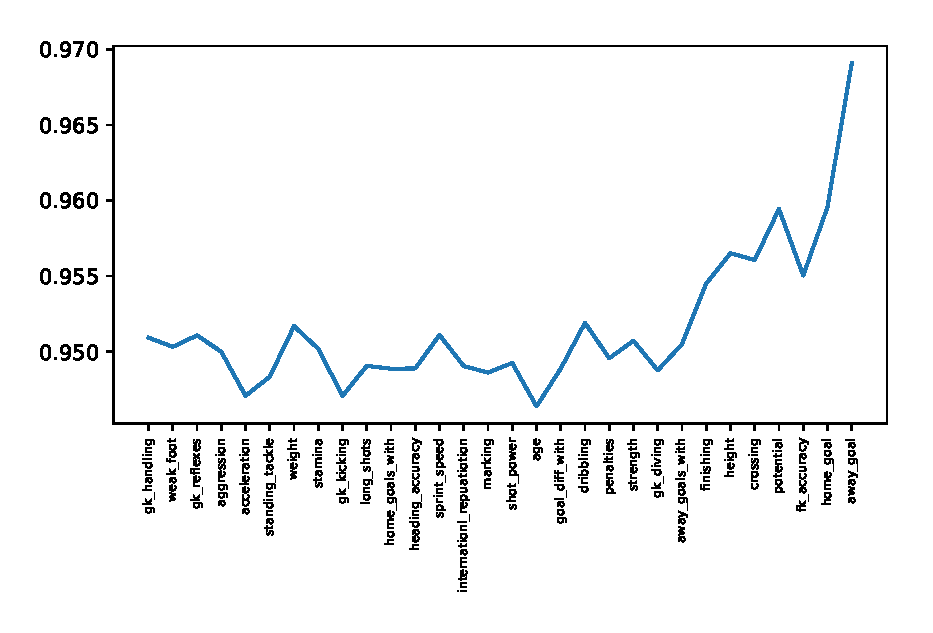
\includegraphics[width=0.7\textwidth]{img/default_avg_lloss.eps}
    \caption{Mean log loss for recursive feature elimination on outcome model with default parameters. Only features from first round to the 30th round are list to ensure figure's readability.}
    \label{fig:def_avg_loss}
\end{figure}

\begin{figure}[H]
    \centering
    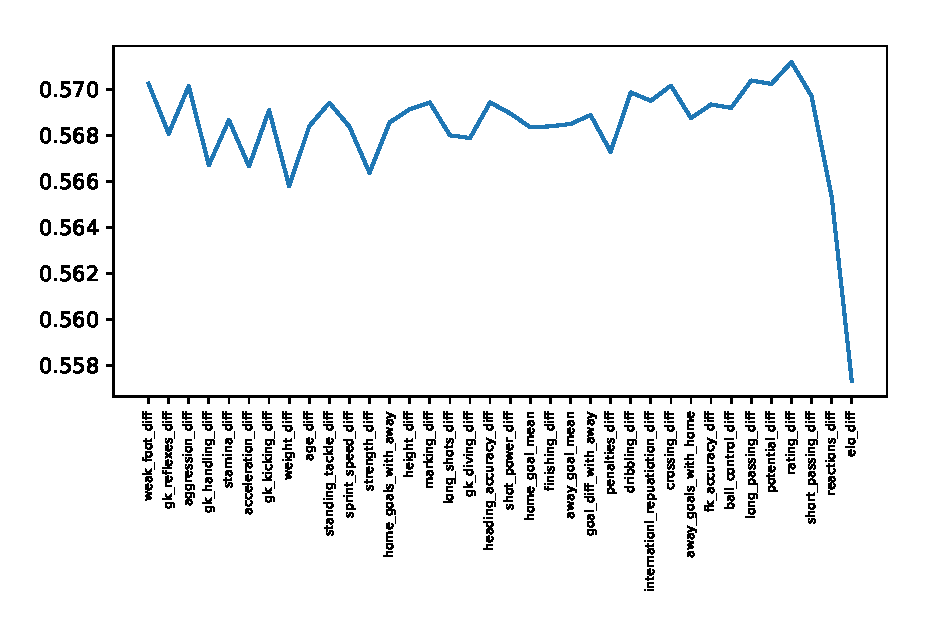
\includegraphics[width=0.7\textwidth]{img/optimal_avg_accuracy.eps}
    \caption{Mean accuracy for recursive feature elimination on outcome model with optimal parameters for all features setup in the table \ref{table:outcomemodel}.}
    \label{fig:optimal_avg_accu}
\end{figure}

\begin{figure}[H]
    \centering
    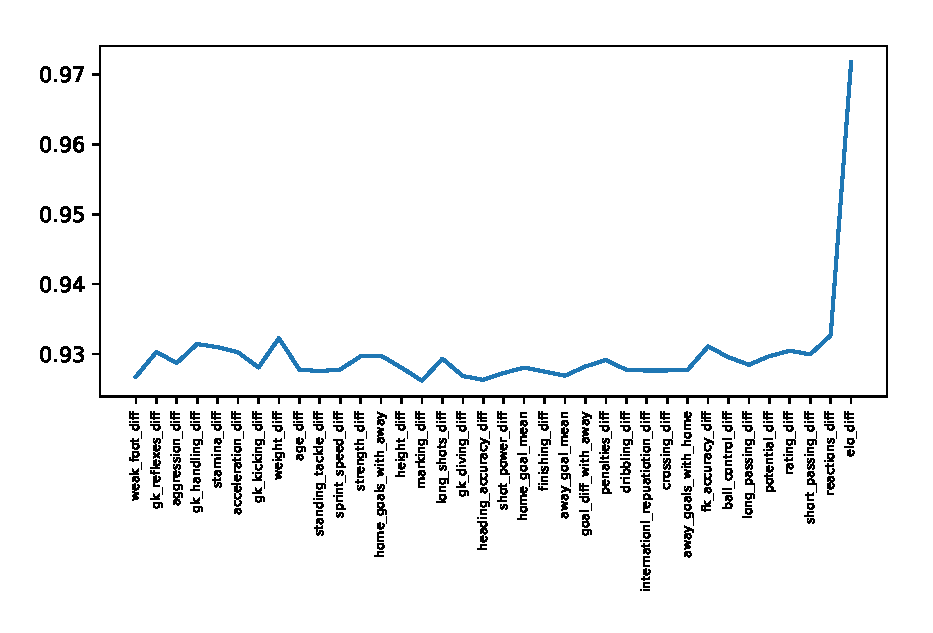
\includegraphics[width=0.7\textwidth]{img/optimal_avg_lloss.eps}
    \caption{Mean log loss for recursive feature elimination on outcome model with optimal parameters for all features setup in the table \ref{table:outcomemodel}.}
    \label{fig:optimal_avg_loss}
\end{figure}

\begin{table}
    \caption{Results for Outcome model with limited features from RFE.}
    \begin{tabular}{| c | c| c| c|c|}
        \hline
        Metric& \textbf{WC 2018} & \textbf{WC 2014} & \textbf{WC 2010} & Mean\\
        \hline
        Accuracy  & 52.97\% $\pm$ 2.36 & 59.69\% $\pm$ 2.3 & 56.09\% $\pm$ 2.47& 56.25 \\
        Log Loss & 0.9953 $\pm$ 0.0087 & 0.9282 $\pm$ 0.0061 & 0.9743 $\pm$ 0.0069& 0.9659 \\
        Unit profit  & -1.79\% $\pm$ 6.16 & 14.12\% $\pm$ 6.02 & 8.82\% $\pm$ 7.47& 7.05 \\
        Kelly profit  & -37.19\% $\pm$ 11.43 & 61.45\% $\pm$ 15.42 & 77.87\% $\pm$ 12.98& 34.04 \\
 \hline
    \end{tabular}
    \label{table:outcomemodel_rfe}
\end{table}

\begin{table}
    \caption{Optimal hyperparameters for Outcome model trained with RFE feature set.}
    \begin{tabular}{| c | c| c| c|}
        \hline
         \# of predictors & Min samples at leaf & Max depth\\
        \hline
         $\sqrt{M}$ & 10 & Na \\
        \hline
    \end{tabular}
    \label{table:hyperparam_results_rfe}
\end{table}


\subsection{Match-level betting activity - what drives the profits?}

